\documentclass[conference]{IEEEtran}
\IEEEoverridecommandlockouts
% The preceding line is only needed to identify funding in the first footnote. If that is unneeded, please comment it out.
\usepackage{cite}
\usepackage{amsmath,amssymb,amsfonts}
\usepackage{algorithm}
\usepackage{algorithmic}
\usepackage{graphicx}
\graphicspath{{evals/data/metrics/figures/final/}}
\usepackage{textcomp}
\usepackage{xcolor}
\usepackage{array}
\usepackage{booktabs}
\usepackage[most]{tcolorbox}

% Churkin Protocol: Color Palette (Harmonious & Minimal)
\definecolor{churkinpurple}{RGB}{94,45,121}    % #5E2D79 (for State)
\definecolor{statusgreen}{RGB}{34,139,34}      % #228B22 (Green for True - Success)
\definecolor{statusred}{RGB}{255,99,71}       % #FF6347 (Light Red/Tomato for False - Stop/Suppressed)
\def\BibTeX{{\rm B\kern-.05em{\sc i\kern-.025em b}\kern-.08em
    T\kern-.1667em\lower.7ex\hbox{E}\kern-.125emX}}

\begin{document}

\title{EXAIM: Explainable AI Middleware for Real-Time Multi-Agent Clinical Decision Support}

\author{\IEEEauthorblockN{Abem Woldesenbet}
\IEEEauthorblockA{\textit{The Beacom College of Computer \& Cyber Sciences} \\
\textit{Dakota State University}\\
Madison, SD, USA \\
abem.woldesenbet@trojans.dsu.edu}
\and
\IEEEauthorblockN{Andy Behrens}
\IEEEauthorblockA{\textit{Information Systems, College of Business \& Information Systems} \\
\textit{Dakota State University}\\
Madison, SD, USA \\
andy.behrens@dsu.edu}
}

\maketitle

\begin{abstract}
 Clinical decision support systems (CDSS) employing multi-agent architectures achieve high diagnostic performance but face a critical transparency bottleneck: they generate verbose, interleaved reasoning traces that are difficult for clinicians to interpret in real time. We present EXAIM (Explainable AI Middleware), an IT artifact developed under a design science research paradigm that transforms live reasoning streams into structured, concise summaries. EXAIM addresses the transparency-usability gap through three primitives: TokenGate for syntax-aware stream regulation, BufferAgent for semantic event detection, and SummarizerAgent for schema-constrained synthesis aligned with clinical frameworks (SBAR/SOAP) \cite{haig2006sbar,podder2023soap}. In contrast to post-hoc methods, EXAIM operates incrementally, triggering updates based on information novelty rather than fixed intervals. We evaluate the artifact through systematic ablation, parameter calibration, and trace-level analysis on 40 diagnostic cases, verifying that event-driven summarization improves semantic coverage relative to structural baselines while reducing redundant updates.
\end{abstract}

\begin{IEEEkeywords}
Clinical decision support systems, explainable artificial intelligence, multi-agent systems, large language models, real-time summarization, middleware architecture, human-AI collaboration
\end{IEEEkeywords}

\section{Introduction}

The integration of multi-agent large language model (LLM) architectures into clinical decision support systems (CDSS) for text-based diagnostic reasoning introduces a critical transparency paradox. While these systems enhance diagnostic accuracy by decomposing reasoning across specialized agents \cite{chenx2025diagnostic,chen2025enhancing}, they generate high-velocity, interleaved reasoning traces that create three fundamental usability barriers: (1) \textbf{Information Overload}, where verbose agent discourse overwhelms clinician cognitive capacity \cite{peng2025tree}; (2) \textbf{Structural Misalignment}, where turn-based output abstractions fail to capture semantic boundaries in streaming reasoning \cite{wu2025incremental}; and (3) \textbf{Interpretability Gaps}, where raw traces obscure the synthesized clinical picture required for rapid decision-making \cite{hong2024argmed,abbas2025xai}.

To address these challenges, we develop EXAIM (Explainable AI Middleware), an IT artifact constructed under a design science research (DSR) paradigm that transforms opaque multi-agent text streams into transparent, clinically actionable summaries.

EXAIM achieves this transformation through three architectural innovations: (1) \textbf{Syntax-Aware Stream Regulation (TokenGate)}, which segments bursty token streams into coherent linguistic units to prevent fragmentation; (2) \textbf{Semantic Event Detection (BufferAgent)}, which filters updates based on completeness, relevance, and novelty to reduce redundant interruptions; and (3) \textbf{Schema-Constrained Synthesis (SummarizerAgent)}, which enforces strict output contracts aligned with SBAR/SOAP communication standards to guarantee consistent interface utility.

The following research question guides the evaluation of this artifact:

\textbf{RQ1:} Can event-driven, schema-constrained summarization improve trace utility by increasing semantic coverage while reducing redundant updates?

We operationalize RQ1 through four sub-questions corresponding to distinct evaluation dimensions:
\begin{itemize}
\item \textbf{RQ1a:} Does EXAIM improve trace coverage under identical schema and peer-summary character constraints compared to structural triggers?
\item \textbf{RQ1b:} Does EXAIM reduce redundant and low-novelty updates through semantic buffering and novelty filtering?
\item \textbf{RQ1c:} Does EXAIM preserve contract-grounded faithfulness when limited continuity across summaries is permitted?
\item \textbf{RQ1d:} What impact does semantic event detection introduce relative to simpler triggers such as turn boundaries or fixed-interval chunking?
\end{itemize}

Throughout the evaluation, "length constraints" are operationalized using a fixed reading-budget proxy introduced in Section IV to enable reproducible comparisons across variants.

This paper makes the following contributions:
\begin{itemize}
\item \textbf{We develop a modular middleware architecture} that transforms streaming multi-agent reasoning traces into structured, clinician-aligned summaries, addressing the cognitive load gap in real-time CDSS.
\item \textbf{We introduce a semantic buffering mechanism} that detects topic shifts, novelty, and critical clinical events to trigger summaries based on context, thereby reducing irrelevant interruptions relative to turn-based baselines.
\item \textbf{We demonstrate process-level transparency} through structured summaries aligned with SBAR/SOAP communication patterns, designed to preserve agent attribution and uncertainty while enforcing strict brevity constraints.
\item \textbf{We formalize the impact of semantic buffering} on coverage, redundancy, faithfulness, and computational cost through a systematic ablation study on 40 diagnostic cases.
\end{itemize}

The remainder of this paper is organized as follows. Section II positions EXAIM within the XAI-CDSS and streaming summarization literature and synthesizes design gaps. Section III details the DSR-guided artifact, its three modules, and provides a demonstrative case walkthrough. Section IV describes the trace replay dataset, calibration procedure, and ablation experiments, reporting quantitative results. Section V interprets findings via design implications and deployment considerations. Section VI concludes and outlines future work.

\section{Literature Review}
\subsection{Clinical Decision Support Systems and Explainability}
Clinical decision support systems (CDSS) have demonstrated potential to improve diagnostic accuracy and patient safety \cite{sutton2020cdss,miyachi2023learning}, yet their real-world adoption remains constrained by usability and workflow integration challenges \cite{derksen2025cdss,bayor2025cdss,harrison2022patient}. Prior studies emphasize that excessive alerting, poor timing, and opaque system behavior contribute to clinician frustration and alert fatigue, limiting trust and sustained use \cite{marcilly2018alerts}. As CDSS increasingly incorporate machine learning and large language models (LLMs), explainability has emerged as a critical requirement for safe deployment in clinical environments \cite{abbas2025xai,chen2025enhancing,hong2024argmed,salimiparsa2021design,sutton2020cdss}. A recent systematic review of CDSS design emphasizes that effective systems must balance clinical accuracy with usability, integration, and transparency \cite{bayor2025cdss}.

\subsubsection{Post-Hoc XAI Methods and Their Limitations}
Explainable AI (XAI) approaches in CDSS have largely focused on post-hoc interpretation methods. Feature importance techniques, including LIME and SHAP, generate local explanations by perturbing inputs and measuring output sensitivity \cite{abbas2025xai,salimiparsa2021design}. Gradient-based visualization methods, such as GradCAM, highlight salient input regions influencing predictions \cite{goel2022covid}. Surrogate model approaches approximate complex models with interpretable alternatives \cite{ribeiro2016lime,guidotti2018survey}.

Frameworks for evaluating XAI systems emphasize the importance of both technical performance and user-centered criteria, suggesting that effective explainability requires consideration of information presentation, cognitive load, and task alignment \cite{vilone2021explainable}. However, these post-hoc methods face critical limitations in real-time clinical workflows. They are poorly aligned with time-sensitive decision-making \cite{abbas2025xai,salimiparsa2021design}, exposing internal model mechanics rather than the evolving clinical narrative \cite{benzion2025anxiety,salimiparsa2021design,hong2024argmed}.

\subsubsection{Cognitive Load and Information Overload}
Traditional explainability approaches fail to account for distributed reasoning and high-velocity, redundant trace emissions that increase output volume and cognitive overload in clinicians \cite{sanwal2025layered,hong2024argmed}. Recent work emphasizes that AI systems for general practice must address cognitive load through transparency that supports clinical sensemaking rather than exposing internal model mechanics \cite{hor2025design}. The update frequency in clinician-facing interfaces often results in verbose or redundant information that does not reflect the summarized treatment plan \cite{wu2025incremental}.

\subsubsection{Clinician Preference for Narrative Explanations}
Empirical studies show that clinicians often prefer concise, narrative explanations grounded in clinical reasoning over probabilistic or feature-based explanations in time-sensitive contexts \cite{silva2023xai}. This misalignment between existing XAI techniques and clinical information needs motivates alternative approaches to explainability that prioritize process transparency and clinical understanding \cite{abbas2025xai,schoonderwoerd2021patterns,salimiparsa2021design,hong2024argmed,derksen2025cdss}. While XAI methods address model interpretability challenges, multi-agent architectures introduce additional complexity in distributing and coordinating explainable reasoning across specialized components.

\subsection{Multi-Agent Systems for Clinical Reasoning}
Multi-agent LLM architectures have gained traction as a means of decomposing complex clinical reasoning tasks across specialized agents responsible for information retrieval, hypothesis generation, verification, and safety assessment \cite{hong2024argmed,ozgun2025psychotherapy,chen2025enhancing}. Prior work demonstrates that distributing reasoning across agents can improve diagnostic performance, robustness, and oversight compared to monolithic models \cite{chenx2025diagnostic,chen2025enhancing,hong2024argmed,peng2025tree}. These systems also offer theoretical advantages for transparency, as individual agents can be assigned interpretable roles within the diagnostic process \cite{ozgun2025psychotherapy}. However, multi-agent systems introduce new explainability challenges. Agent interactions generate long, interleaved reasoning traces that include exploratory hypotheses, internal deliberation, and repetitive grounding statements \cite{hong2024argmed}. While some systems explicitly expose agent reasoning to users, these traces are typically verbose and require post-hoc review, limiting their practical utility during live clinical decision-making. Existing multi-agent frameworks largely assume that transparency is achieved by exposing reasoning in full, rather than by managing how and when information is presented to clinicians \cite{wu2025incremental,leduc2025speech,schneider2024meeting}. The verbosity of multi-agent reasoning traces is compounded by interface design choices, particularly turn-based interaction paradigms that misalign with semantic completeness.

\subsection{Turn-Based Interfaces and Streaming Reasoning}

\subsubsection{Limitations of Turn-Based Paradigms}
Most conversational and multi-agent AI systems adopt turn-based interaction paradigms, surfacing outputs only when an agent completes a turn. This abstraction is inherited from human dialogue systems, where turn-taking often corresponds to semantic completion. However, in multi-agent LLM systems, a single turn may contain multiple topic shifts, partial inferences, or exploratory reasoning branches. Treating turns as semantic units can therefore result in lossy compression, redundancy, and reduced faithfulness when summarization is applied. When multi-agent reasoning traces are compressed at turn boundaries, semantically incomplete fragments may be forced into summaries, while complete reasoning spans crossing turn boundaries may be artificially split. This leads to information loss, as partial hypotheses and exploratory statements are either omitted or presented without sufficient context.

\subsubsection{Semantic Boundary Detection in Streaming Systems}
Recent work on streaming and incremental reasoning highlights the limitations of turn-based interfaces in high-velocity information environments \cite{leduc2025speech,wu2025incremental}. Studies in meeting summarization demonstrate that incremental updates triggered by semantic boundaries rather than fixed intervals improve information retention and regularize update frequency \cite{schneider2024meeting}. Similar findings emerge in customer support and medical dialogue systems, where content-based triggering outperforms interval-based approaches. These findings suggest that real-time systems require adaptive mechanisms to regulate information flow based on content semantics rather than generation structure. For multi-agent clinical decision support, this implies that summarization triggers should be driven by semantic completeness, clinical relevance, and novelty rather than arbitrary turn boundaries or fixed time intervals.

Addressing these interface challenges requires not only semantic event detection but also structured presentation formats aligned with clinical communication practices and documentation standards.



\subsection{Clinical Summarization and Structured Communication}
Clinical summarization research provides important foundations for managing information overload in healthcare settings \cite{vanveen2023summarization,leduc2025speech,yim2023acibench,krishna2021soap}.

\subsubsection{Clinical Communication Frameworks}
Structured summaries aligned with clinical documentation standards, such as SBAR (Situation-Background-Assessment-Recommendation) and SOAP (Subjective-Objective-Assessment-Plan), support predictable, scannable presentation formats \cite{haig2006sbar,podder2023soap}. These frameworks reduce communication errors and support clinical handoff processes \cite{krishna2021soap,zhang2024annotate}. The SBAR framework structures information into four components: current situation, relevant background context, clinical assessment, and recommended actions. SOAP notes organize clinical encounters into subjective patient reports, objective measurements, diagnostic assessment, and treatment plans. Both frameworks emphasize brevity, actionability, and role-appropriate information density.

\subsubsection{LLM-Based Clinical Summarization}
Large language models have shown strong performance in generating clinical summaries when explicit length and structure constraints are enforced \cite{vanveen2023summarization}. Recent work on LLM-based clinical dialogue summarization has validated the use of expert clinician evaluation for assessing summary quality, emphasizing faithfulness, completeness, and clinical utility as key evaluation criteria \cite{fraile2025llm}.

\subsubsection{Streaming and Real-Time Summarization}
Recent studies indicate that streaming summarization can outperform post-hoc summarization by preserving context and reducing the need for retrospective compression \cite{bailly2025divide}. Additionally, token filtering strategies have been proposed to reduce redundancy in clinical texts \cite{piya2025contextual}. However, most clinical summarization systems operate on completed conversations or documents and do not address the challenges posed by multi-agent reasoning streams \cite{wu2025incremental,schneider2024meeting}. Specifically, they assume a single narrative source rather than multiple interacting agents producing overlapping and partially redundant content. Human-in-the-loop dialogue systems literature emphasizes the importance of faithfulness and coherence as critical evaluation dimensions for interactive systems \cite{chen2022hitl}. To our knowledge, prior systems do not jointly perform semantic event triggering over interleaved multi-agent traces and emit clinician-aligned schema summaries. EXAIM integrates concepts from XAI, clinical summarization, and streaming systems by introducing a dedicated middleware layer that regulates information flow, detects meaningful reasoning events, and generates clinician-aligned summaries in real time. % Added positioning statement

\section{Artifact Description}

Design Science aims to create and evaluate IT artifacts intended to solve identified organizational problems \cite{hevner2004design}. Consistent with the principles of DSR, we develop EXAIM as a solution-oriented IT artifact designed to address the specific problem of cognitive overload in multi-agent CDSS. This approach aligns with recent applications of DSR for developing AI-based clinical tools that balance technical innovation with practical usability requirements \cite{hor2025design}. Following the process model outlined by Peffers et al. \cite{peffers2007dsr}, this section provides a systematic description of the artifact's architecture, key components, and operational logic. We first present the overall framework, then detail the three primary modules (TokenGate, BufferAgent, SummarizerAgent), and finally demonstrate the system's operation through a case walkthrough.

\begin{figure*}[htbp]
\centering
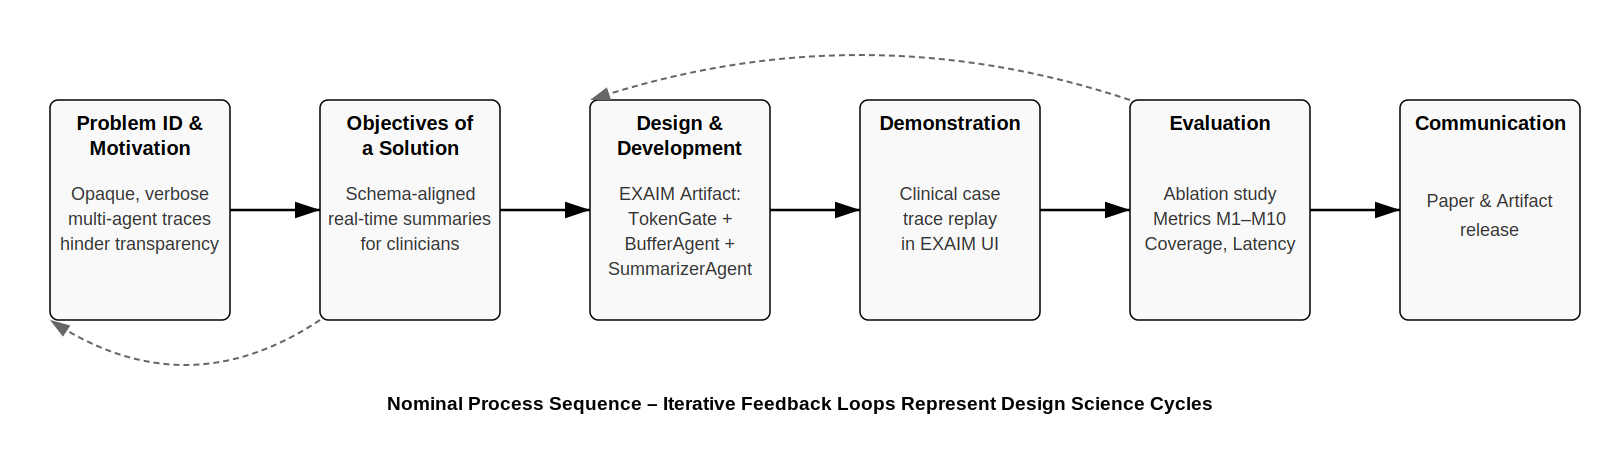
\includegraphics[width=\textwidth]{dsr/DSR.pdf}
\caption{EXAIM Design Science Research Methodology (DSRM) process model showing the six stages of our research lifecycle and the process iteration feedback loops.}
\label{fig:dsr}
\end{figure*}

\subsection{Overall Framework}
\label{sec:overall-framework}

EXAIM functions as a transparency middleware that sits between upstream diagnostic multi-agent systems and downstream clinician-facing interfaces. The core architectural challenge is straightforward: multi-agent systems generate thousands of token-level deltas per diagnostic session, yet clinicians require at most a dozen discrete, structured updates. EXAIM bridges this gap by transforming high-velocity, interleaved token streams into semantically bounded summary events.

As illustrated in Figure~\ref{fig:system-architecture}, the system accepts an asynchronous stream of token deltas $D = \{(a_t, \tau_t)\}_{t=1}^T$, where each delta consists of an agent identifier $a_t$ and a text fragment $\tau_t$. This input model is deliberately agnostic to the underlying agent architecture---EXAIM requires only that agents emit text incrementally, making it compatible with any streaming LLM framework.

The system emits a sequence of structured summary objects $S = \{s_1, s_2, \ldots, s_N\}$, where each $s_i$ conforms to a strict JSON schema mapped to clinical communication standards (SBAR/SOAP). Critically, $N \ll T$, representing a meaningful reduction in event frequency.

\subsubsection{Design Objectives}
\label{sec:design-objectives}
Four explicit design objectives constrain the system's behavior and provide the criteria against which ablation variants are evaluated:

\begin{enumerate}
\item \textbf{DO1 (Update Budget):} Prefer fewer, higher-information summaries per case to respect clinician cognitive load and interruption costs. We therefore treat update frequency as a constrained resource and evaluate methods under an explicit update budget; approaches that require high-frequency updates are unlikely to be usable in time-pressured clinical workflows, even when they increase raw coverage.
\item \textbf{DO2 (Schema Contract):} Strict schema compliance with bounded character budgets to guarantee stable UI footprint. All outputs must validate against the AgentSummary schema or be discarded.
\item \textbf{DO3 (Non-Blocking Observation):} Middleware processing occurs asynchronously in a ``sidecar'' pattern, ensuring EXAIM's analysis never adds latency to the upstream diagnostic process.
\item \textbf{DO4 (Strict Grounding):} Summaries generated solely from buffered trace content and limited history ($k=3$ prior summaries), explicitly prohibiting external knowledge retrieval.
\end{enumerate}

These constraints reflect a fundamental design philosophy: EXAIM does not attempt to ``improve'' the diagnostic reasoning but rather to make it transparently observable.

\begin{figure*}[htbp]
    \centering
    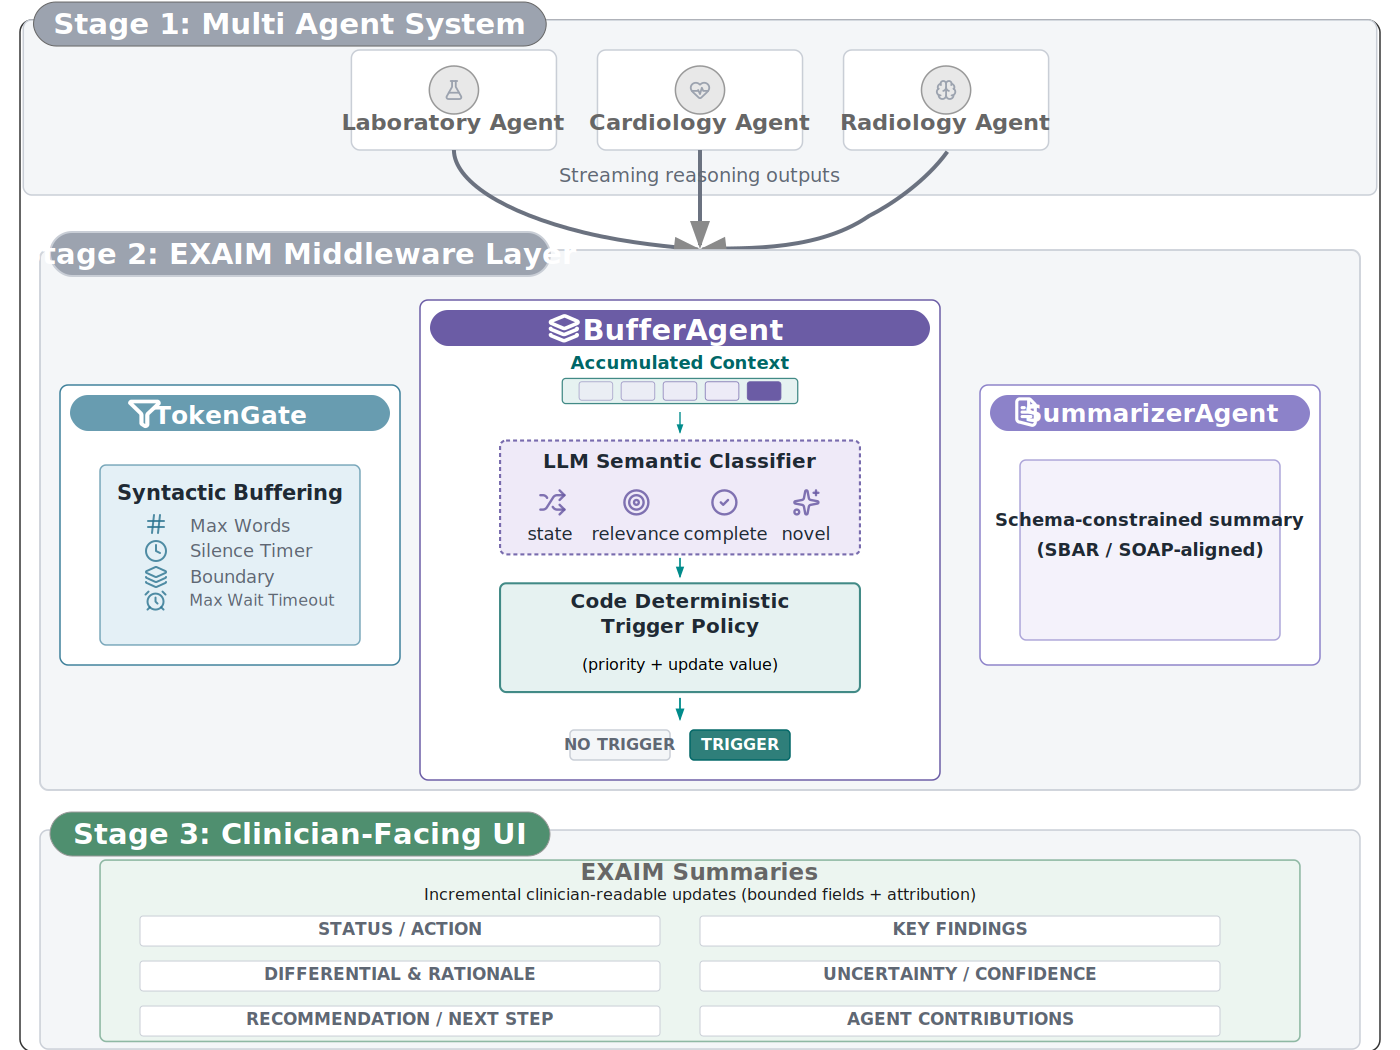
\includegraphics[width=\textwidth]{../raw/systemFigure/system.pdf}
    \caption{EXAIM System Architecture showing the three-stage pipeline: (1) Interleaved Input Stream from multi-agent sources, (2) EXAIM Middleware Layer with TokenGate (syntax-aware buffering), BufferAgent (semantic event detection), and SummarizerAgent (schema-constrained synthesis), and (3) Structured Output in SBAR/SOAP format for clinician-facing interfaces.}
    \label{fig:system-architecture}
\end{figure*}


\subsection{TokenGate: Syntax-Aware Stream Regulation}

Raw LLM token streams arrive in unpredictable bursts. In a typical multi-agent diagnostic session, a single agent might emit individual characters during deliberation, then suddenly flush complete paragraphs when reaching a conclusion. This fragmentation creates a fundamental challenge for semantic analysis: to detect topic shifts or assess novelty, the system requires coherent linguistic units---complete clauses or sentences---but the raw stream provides no such boundaries.

TokenGate addresses this gap by functioning as a stateful accumulation buffer with intelligent flush triggers. Rather than forwarding every delta immediately to the semantic analyzer, it accumulates incoming text until a syntactically meaningful boundary is reached. The component operates on a priority-based policy with four trigger conditions, designed to balance linguistic coherence against latency guarantees:

\begin{enumerate}
\item \textbf{Boundary-Aware Flush}: When the buffer contains at least $w_{\text{min}}$ words AND ends with sentence-terminal punctuation (period, question mark, exclamation), the system flushes immediately. This represents the ideal case---a complete, grammatical unit ready for semantic analysis.

\item \textbf{Hard Limit}: If the buffer exceeds $w_{\text{max}}$ words regardless of punctuation, a forced flush occurs. This prevents pathological memory growth when agents generate long unpunctuated streams (e.g., extended medical histories or literature reviews).

\item \textbf{Silence Timeout}: If the agent goes silent for more than $t_{\text{silence}}$ seconds AND the buffer contains at least $w_{\text{min}}$ words, the system flushes. This captures the common pattern where agents ``pause'' between reasoning steps without emitting explicit punctuation.

\item \textbf{Safety Valve}: If total wait time exceeds $t_{\text{max}}$ seconds since the first delta arrived, the system flushes regardless of buffer state. This guarantees liveness---the system will never deadlock waiting for a boundary that may never arrive.
\end{enumerate}

These parameters ($w_{\text{min}}$, $w_{\text{max}}$, $t_{\text{silence}}$, $t_{\text{max}}$) jointly determine the Pareto frontier between linguistic coherence and real-time responsiveness. Section IV-B describes the systematic calibration procedure used to identify optimal values.

\subsection{BufferAgent: Semantic Event Detection}

If TokenGate solves the syntactic segmentation problem, BufferAgent solves the semantic filtering problem. Not every coherent chunk of agent reasoning deserves to interrupt the clinician. An agent might spend several sentences re-stating background knowledge, concurring with a previous diagnosis, or exploring a hypothesis already ruled out by others. Presenting all such content as discrete updates would recreate the very cognitive overload EXAIM aims to prevent.

BufferAgent acts as the system's cognitive filter, analyzing each chunk from TokenGate to determine whether it merits triggering a summary. The decision process operates in two stages, deliberately separating semantic interpretation (performed by an LLM) from control logic (executed by deterministic code). This separation ensures that while the system leverages language model capabilities for content understanding, the final trigger decision remains auditable and explainable.

When a chunk $C$ arrives, BufferAgent invokes an LLM classifier to extract four semantic predicates: \textbf{Complete}, \textbf{Relevant}, \textbf{Novel}, and \textbf{State} (continuation, topic shift, or critical alert). These feed a deterministic trigger decision:
\[
T = \begin{cases}
\text{True} & \text{if } \mathit{State} = \text{CRITICAL} \\
\text{True} & \text{if } \mathit{Complete} \land \mathit{Relevant} \land \mathit{Novel} \\
\text{True} & \text{if } (\mathit{State} = \text{SHIFT}) \land \mathit{Relevant} \land \mathit{Novel} \\
\text{False} & \text{otherwise}
\end{cases}
\]
This encodes a hypothesis that clinicians need immediate critical alerts, comprehensive novel conclusions, and topic transitions---but not incremental deliberation or redundant restatements.

\subsection{SummarizerAgent: Schema-Constrained Synthesis}

When BufferAgent determines that a chunk merits clinician attention, SummarizerAgent faces the final transformation challenge: compressing potentially verbose agent reasoning into a rigid, scannable format aligned with clinical communication standards. This component embodies the system's commitment to interface stability---no matter how chaotic or verbose the upstream reasoning, the output must conform to a bounded schema that downstream UIs can reliably render.

The agent receives three inputs: the triggering chunk $C$, the agent context (identifier and role), and a sliding window of the three most recent summaries $H_{k=3}$. This limited history serves dual purposes---it enables the summarizer to avoid repeating recently stated information while providing continuity for multi-turn reasoning threads.

Generation employs a three-attempt validation strategy. First, \textbf{Initial Generation}: the LLM generates structured output using strict Pydantic type definitions with schema enforcement (strict=True) mapped to SBAR/SOAP fields (Table~\ref{tab:schema}). Second, \textbf{Retry with Rewrite}: if character limits are exceeded, the system creates a targeted rewrite prompt identifying the violating fields and their required length reductions, then re-invokes the LLM. Third, \textbf{Fallback Truncation}: if validation still fails after the rewrite attempt, the system applies hard truncation at character boundaries to ensure schema compliance.

This schema-first approach differs fundamentally from unconstrained summarization. Traditional abstractive summarizers optimize for semantic coverage or fluency but provide no length guarantees. EXAIM inverts this priority: the character budgets are non-negotiable constraints derived from UI layout requirements, while semantic coverage is maximized subject to these bounds.

The AgentSummary schema (Table~\ref{tab:schema}) enforces a structured contract between the middleware and clinician-facing interfaces. Each of the six fields maps directly to elements of SBAR (Situation-Background-Assessment-Recommendation) and SOAP (Subjective-Objective-Assessment-Plan) clinical communication frameworks. Character budgets operationalize qualitative usability principles into deterministic constraints, ensuring that the schema design reflects three core principles: (1) \textit{Scannability}: brief field lengths force summarization to salient points, preventing verbose blocks that impair rapid comprehension; (2) \textit{Clinical Alignment}: field semantics mirror established documentation workflows, reducing cognitive overhead for clinician users; and (3) \textit{Bounded Contracts}: hard character limits guarantee stable UI footprint regardless of model verbosity, preventing layout shifts or overflow in dashboard interfaces.

\begin{table*}[htbp]
\caption{EXAIM Summary Schema: Clinical Mapping and Bounded Output Budgets}
\label{tab:schema}
\begin{center}
\renewcommand{\arraystretch}{1.3}
\begin{tabular}{p{2.5cm}p{2.5cm}p{4cm}p{1.5cm}p{4.5cm}}
\toprule
\textbf{Field} & \textbf{Clinical Map} & \textbf{Role} & \textbf{Budget (Chars)} & \textbf{Design Motivation} \\
\midrule
Status / Action & SBAR: Situation & Alert header; scannable update. & 150 chars & Enforces scannability via brief title heuristic \cite{pourian2025alerts}. \\
Key Findings & SOAP: Obj/Subj & Salient facts; ``live snippet'' paradigm. & 180 chars & Supports $\sim$2 concise snippets aligned with targeted summarization limits \cite{vanveen2023summarization}. Structured presentation addresses transparency barriers identified in patient-centered CDSS deployment \cite{harrison2022patient}. \\
Differential & SOAP: Assessment & Diagnostic interpretation. & 210 chars & Bounds complexity to maintain interpretability \cite{lage2019interpretability}. \\
Uncertainty & SOAP: Assessment & Explicit confidence signal. & 120 chars & Simplified framing for trust calibration \cite{goel2022covid}. \\
Rec. / Plan & SOAP: Plan & Actionable next step. & 180 chars & Action-linked explanations \cite{silva2023xai}. \\
Agent Contrib. & System Meta & Attribution of active agents. & 150 chars & Pipeline transparency patterns \cite{donadello2021sexai}. \\
\bottomrule
\end{tabular}
\end{center}
\footnotesize
Note: Character budgets are hard constraints that enforce a bounded UI contract, ensuring stable interface footprint regardless of model verbosity.
\normalsize
\end{table*}

\subsection{Demonstrative Case Walkthrough}

To demonstrate EXAIM's semantic filtering and redundancy detection mechanisms, we analyze a specific interaction sequence from a multi-agent reasoning trace (Case ID: 3949). This trace was generated using the MAC Framework (described in Section IV-A), which simulates a team of diagnostic agents collaborating on a complex medical case. This example illustrates how the middleware distinguishes between verbose repetition and genuinely novel clinical information.

\textbf{1. Context State (Pre-Condition)} Prior to this segment, doctor0 and doctor1 had already established Spinocerebellar Ataxia (SCA) as the leading diagnosis. The middleware had generated summaries capturing this consensus and the recommended genetic tests (Log ID: summary\_3). The active buffer was empty.

\textbf{2. The Raw Input Stream} doctor2 then enters the discussion. The agent generates a verbose response concurring with the previous agents and re-stating the established diagnosis.

\textit{Raw Trace (doctor2):} ``\textit{\#\#\# Most Likely Diagnosis: Spinocerebellar Ataxia (SCA): I concur with both Doctor0 and Doctor1 that the most likely diagnosis is spinocerebellar ataxia... The gradual onset at age 30 years also aligns with hereditary SCAs... \#\#\# Differential Diagnoses: 1. Multiple Systems Atrophy (MSA): While I agree that MSA typically presents with...}''

\textbf{3. BufferAgent Logic (Internal Rationale)} While the dashboard remained visually static (see Fig.~\ref{fig:suppression-demo}), the middleware was actively analyzing the stream. As visualized in Fig.~\ref{fig:logic-card}, the system detected semantic redundancy through its multi-stage evaluation process. Despite the input's clinical relevance, the novelty check failed, causing the middleware to suppress the update and prevent redundancy.

\begin{figure}[h]
    \centering
    \scalebox{0.75}{%
    \begin{tcolorbox}[
        enhanced,
        colback=white,
        colframe=black,
        boxrule=0.5mm,
        arc=2mm,
        drop shadow,
        left=4mm,
        right=4mm,
        top=2mm,
        bottom=2mm,
        title=\textbf{BufferAgent Status [doctor2]},
        fonttitle=\bfseries\normalsize,
        coltitle=black,
        colbacktitle=white,
        halign title=center,
        fontupper=\normalsize
    ]
        \normalsize
        
        \textbf{Input Stream:}
        \vspace{-1mm}
        \begin{quote}
            \itshape "...I concur with both Doctor0 and Doctor1... adding no new information."
        \end{quote}
        \vspace{1.5mm}
        
        \textbf{Decision Flags:}
        \vspace{0.5mm}
        
        \begin{center}
        \begin{tabular}{@{}c@{}}
            \raisebox{5pt}{State} \\
            \tcbox[colback=churkinpurple!15, colframe=churkinpurple, size=small, boxrule=0.5mm, left=2mm, right=2mm, top=0.5mm, bottom=0.5mm, fontupper=\normalsize]{\textcolor{churkinpurple}{\texttt{SAME\_TOPIC\_CONTINUING}}}
        \end{tabular}
        \end{center}
        
        \vspace{0.1mm}
        \begin{center}
        \begin{tabular}{@{}c@{\hspace{2mm}}c@{\hspace{2mm}}c@{}}
            \begin{tabular}{@{}c@{}}
                \raisebox{5pt}{Complete} \\[-3pt]
                \tcbox[colback=statusgreen!15, colframe=statusgreen, size=small, boxrule=0.5mm, left=2mm, right=2mm, top=0.2mm, bottom=0.2mm, fontupper=\normalsize]{\textcolor{statusgreen}{\textbf{True}}}
            \end{tabular} &
            \begin{tabular}{@{}c@{}}
                \raisebox{5pt}{Relevant} \\[-3pt]
                \tcbox[colback=statusgreen!15, colframe=statusgreen, size=small, boxrule=0.5mm, left=2mm, right=2mm, top=0.2mm, bottom=0.2mm, fontupper=\normalsize]{\textcolor{statusgreen}{\textbf{True}}}
            \end{tabular} &
            \begin{tabular}{@{}c@{}}
                \raisebox{5pt}{Novel} \\[-3pt]
                \tcbox[colback=statusred!15, colframe=statusred, size=small, boxrule=0.5mm, left=2mm, right=2mm, top=0.2mm, bottom=0.2mm, fontupper=\normalsize]{\textcolor{statusred}{\textbf{False}}}
            \end{tabular} \\
        \end{tabular}
        \end{center}
        \vspace{-2mm}
        \begin{center}
            $\downarrow$
        \end{center}
        \vspace{-2mm}
        \begin{center}
            \tcbox[
                enhanced,
                colback=statusred!20,
                colframe=statusred,
                boxrule=0.5mm,
                size=normal,
                fontupper=\bfseries\normalsize,
                left=3mm,
                right=3mm,
                top=0.5mm,
                bottom=0.5mm
            ]{\textcolor{statusred}{Trigger = False (Suppressed)}}
        \end{center}
        
        \vspace{0.1mm}
        \noindent\rule{\linewidth}{0.5mm}
        \vspace{0.5mm}
        
        \textbf{Rationale:} Doctor2 concurs with SCA based on ataxia/dysarthria/MRI... adding no new information. The content is \textcolor{statusgreen}{relevant} as it details planned actions, but it is \textcolor{statusred}{not novel} as these details were already broadly mentioned in previous summaries.
    \end{tcolorbox}%
    }
    \caption{BufferAgent System Status Card showing the hierarchical decision logic. Three evaluation conditions (\textcolor{statusgreen}{Complete=True}, \textcolor{statusgreen}{Relevant=True}, \textcolor{statusred}{Novel=False}) combine to produce the final result: \textcolor{statusred}{Trigger=False (Suppressed)}, preventing redundant update generation.}
    \label{fig:logic-card}
\end{figure}

\begin{figure*}[htbp]
\centering
\scalebox{1}{%
\includegraphics[width=\textwidth]{case_walkthrough/CaseWalkthroughImage.png}%
}
\caption{The EXAIM dashboard during redundancy suppression. The left panel shows the raw, verbose stream from doctor2 concurring with the diagnosis. The right panel remains static (displaying the previous doctor1 update), visually confirming that the middleware successfully filtered the non-novel content.}
\label{fig:suppression-demo}
\end{figure*}

\textbf{4. Outcome} Consequently, EXAIM filtered this update, preventing the generation of a low-value summary. The middleware continued to buffer doctor2's subsequent tokens silently until the agent introduced specific new details regarding ``High-Resolution MRI techniques'' and ``Oligoclonal bands,'' which finally triggered a consolidated, high-density update.

\section{Experiments and Results}

We verify the effectiveness of the EXAIM artifact through a "glass-box" evaluation methodology using deterministic replays of multi-agent reasoning traces. This approach allows us to stress-test the middleware's flow-control capabilities independent of variations in upstream agent behavior.

\textbf{Evaluation Objectives}: We aim to experimentally confirm that:
\begin{enumerate}
    \item EXAIM's syntax-aware segmentation and semantic buffering improve information coverage compared to structural baselines (Validating RQ1a).
    \item The novelty detection mechanism reduces redundant updates without sacrificing essential clinical information (Validating RQ1b).
    \item The schema-constrained synthesis preserves faithfulness despite aggressive summarization (Validating RQ1c).
    \item Component-level ablation demonstrates the necessity of the complete three-primitive architecture (Validating RQ1d).
\end{enumerate}

\subsection{Data / Trace Replay Setup}

We utilized the Multi-Agent Conversation (MAC) framework \cite{chenx2025diagnostic} as the upstream trace generator. MAC is a multi-agent diagnostic system where diverse doctor agents and a supervisor collaborate to solve complex medical cases. We executed MAC with GPT-4o-mini using the authors' default configuration without modification. To capture realistic streaming dynamics, we instrumented MAC via a transparent OpenAI API monkeypatch that logs per-delta emissions and microsecond timestamps without altering MAC's conversation logic, speaker selection, or termination behavior. These logs serve as a frozen replay dataset of 40 rare-disease diagnostic cases from MAC's dataset (seed=42), enabling deterministic simulation of live streams.

\subsection{Calibration Protocol}

To ensure fair evaluation, we executed a rigorous parameter selection process before final testing:
\begin{enumerate}
    \item \textbf{TokenGate Calibration}: We performed a grid search over 625 policy combinations (varying word counts and timeouts) on the replay dataset. The final policy (min\_words=60, max\_word=100, silence=1.0s, safe\_wait=4.0s) was selected via Pareto frontier analysis to jointly optimize latency and linguistic coherence.
    \item \textbf{V3 Fixed-Chunk Calibration}: V3 chunk size was derived from V0 TokenGate regular flushes (excluding end-of-trace and turn-end) using a two-stage median: per-case median CTU, then median across the first 40 cases. This ensures V3 operates at comparable segmentation granularity to V0 while isolating the contribution of adaptive boundaries.
    \item \textbf{Measurement Standardization}: We report all token volumes and costs in \textbf{Character-Normalized Token Units (CTU)}, defined as $\lceil \text{len(text)} / 4 \rceil$, to ensure vendor-agnostic reproducibility.
\end{enumerate}
Table~\ref{tab:tokengate-grid} details the explored parameter space.

\begin{table}[htbp]
\caption{TokenGate Parameter Calibration Grid}
\begin{center}
\renewcommand{\arraystretch}{1.3}
\begin{tabular}{lc}
\toprule
\textbf{Parameter} & \textbf{Values Tested} \\
\midrule
min\_words & 30, 40, 50, 60, 70 \\
max\_words & 80, 100, 120, 140, 160 \\
silence\_timer (seconds) & 1.0, 1.5, 2.0, 2.5, 3.0 \\
max\_wait\_timeout (seconds) & 4.0, 5.0, 6.0, 7.0, 8.0 \\
\bottomrule
\end{tabular}
\label{tab:tokengate-grid}
\end{center}
\end{table}

\subsection{Ablation and Baselines}

We isolate the contribution of each architectural primitive through a controlled ablation study. Table~\ref{tab:ablation-variants} defines the five experimental configurations (V0-V4), designed to test specific hypotheses:
\begin{itemize}
    \item \textbf{V0 (Full EXAIM)} includes all primitives.
    \item \textbf{V1 (Turn-End)} removes TokenGate and BufferAgent, triggering only on agent turn ends (testing the "structural vs. semantic" hypothesis).
    \item \textbf{V2 (No BufferAgent)} removes semantic filtering (testing the necessity of the cognitive filter).
    \item \textbf{V3 (Fixed-Chunk)} replaces TokenGate with fixed intervals (testing the value of syntax-awareness).
    \item \textbf{V4 (No Novelty)} disables the novelty check (testing the redundancy suppression mechanism).
\end{itemize}

\begin{table*}[htbp]
\caption{Ablation Variant Configurations}
\label{tab:ablation-variants}
\begin{center}
\renewcommand{\arraystretch}{1.3}
\begin{tabular}{lccccl}
\toprule
\textbf{Variant} & \textbf{TokenGate} & \textbf{BufferAgent} & \textbf{Novelty} & \textbf{Trigger} & \textbf{Description} \\
\midrule
V0 (Full EXAIM) & \checkmark & \checkmark & \checkmark & Semantic & Complete pipeline with all components \\
V1 (Turn-End) & $\times$ & $\times$ & N/A & Turn boundaries & Baseline: summarize only at turn\_end events \\
V2 (No BufferAgent) & \checkmark & $\times$ & N/A & All TokenGate flushes & Tests impact of semantic filtering \\
V3 (Fixed-Chunk) & $\times$ & \checkmark & \checkmark & Fixed CTU intervals & Calibrated fixed-size chunking \\
& (fixed CTU) & & & & vs. adaptive segmentation \\
V4 (No Novelty) & \checkmark & \checkmark & $\times$ & Semantic & Tests novelty gating impact \\
\bottomrule
\end{tabular}
\end{center}
\footnotesize
Note: All variants use identical SummarizerAgent schema and history\_k=3 for fair comparison.
\normalsize
\end{table*}

\subsection{Metrics}

We prioritized five metrics that directly quantify utility and reliability proxies:

\begin{itemize}
    \item \textbf{Strict Faithfulness (M6b):} The fraction of summary concepts grounded in the full trace:
    \begin{equation}
    M6b = \frac{|\text{summary\_CUIs} \cap \text{trace\_CUIs}|}{|\text{summary\_CUIs}|}
    \end{equation}
    Higher scores indicate stronger concept-level grounding. This metric penalizes unsupported insertions but does not account for semantic paraphrase (see Section IV-C.3). Faithfulness is a standard evaluation criterion in human-in-the-loop dialogue systems \cite{chen2022hitl}.
    \item \textbf{Redundancy Reduction (M3):} Measured via mean Jaccard similarity between consecutive summary updates:
    \begin{equation}
    M3 = \frac{1}{n-1}\sum_{i=1}^{n-1} \frac{|C_i \cap C_{i+1}|}{|C_i \cup C_{i+1}|}
    \end{equation}
    where $C_i$ and $C_{i+1}$ are the sets of unique UMLS concepts (CUIs) extracted from summaries $S_i$ and $S_{i+1}$, and $n$ is the total number of summaries. Lower scores indicate successful suppression of repetitive content.
    \item \textbf{Trace Coverage (M4):} The fraction of unique trace CUIs captured across all summaries:
    \begin{equation}
    M4 = \frac{|\bigcup_{i=1}^{n} \text{summary\_CUIs}_i \cap \text{trace\_CUIs}|}{|\text{trace\_CUIs}|}
    \end{equation}
    This metric is \emph{not normalized by update count}, and therefore inherently favors high-frequency systems. M7 (Budget Efficiency) provides the normalized coverage view.
    \item \textbf{System Latency (M8):} The end-to-end processing time (buffer analysis + summarization generation) to validate the ``real-time'' architectural claim.
    \item \textbf{Schema Compliance (M10):} The rate of successful adherence to the JSON clinical output schema, verifying the system's structural reliability.
\end{itemize}
Supplementary metrics (Update Count, Token Volume, LLM Cost) provide context for trade-off analysis.

\subsubsection{Limitations of Concept-Level Faithfulness Metrics}

Our faithfulness metrics (M6a, M6b) operate at the level of explicit concept realization rather than semantic equivalence or entailment. This introduces a fundamental mismatch: overlap-based metrics like ROUGE fail to correlate with clinical quality when models use paraphrasing rather than literal repetition \cite{fraile2025llm,bailly2025divide}.

Schema-constrained summarization necessarily introduces transformations that reduce recall under strict NER-based concept matching: abbreviation of clinical phrases (e.g., ``acute renal failure'' $\rightarrow$ ``AKI''), normalization of hedged statements and compression omitting modifiers to meet character limits \cite{yim2023acibench}, and schema remapping reorganizing facts into SBAR/SOAP slots through incremental UPDATE and REMOVE operations \cite{zhang2024annotate}.

UMLS-based NER assumes explicit lexical realization and near-literal mention of entities \cite{vanveen2023summarization,yim2023acibench}, misaligning with summaries that preserve semantic content through paraphrase. String-matching approaches demonstrate low correlation with physician preferences when content is normalized or compressed \cite{yim2023acibench,vanveen2023summarization}, causing schema-constrained summarizers to under-score even when accurately representing clinical content \cite{fraile2025llm}.

Despite these limitations, concept-level metrics remain informative for relative comparisons across ablation variants under identical extraction assumptions. Future work should incorporate clinician-judged factual consistency \cite{fraile2025llm}, entailment verification, and task-based evaluation to complement automated assessment.

\subsection{Results}

\subsubsection{Contract and Quality Metrics}
Table~\ref{tab:contract-metrics} reports metrics related to schema compliance, faithfulness, and latency---core indicators of EXAIM's reliability as a clinician-facing interface component. We report bootstrap 95\% confidence intervals (10,000 samples, seed=42) for M4, M6a, and M6b where available.

\begin{table}[htbp]
\caption{Contract and Quality Metrics with Bootstrap 95\% CIs}
\begin{center}
\resizebox{\columnwidth}{!}{%
\renewcommand{\arraystretch}{1.3}
\begin{tabular}{lccccc}
\toprule
\textbf{Metric} & \textbf{V0} & \textbf{V1} & \textbf{V2} & \textbf{V3} & \textbf{V4} \\
\midrule
\multicolumn{6}{l}{\textit{Faithfulness (M6b)}} \\
Mean & 0.421 & 0.333 & 0.409 & 0.382 & 0.424 \\
CI [low, high] & [0.389, 0.453] & [0.309, 0.356] & [0.382, 0.437] & [0.353, 0.413] & [0.395, 0.454] \\
\midrule
\multicolumn{6}{l}{\textit{Window-Groundedness (M6a)}} \\
Mean & 0.825 & 0.787 & 0.879 & 0.823 & 0.845 \\
CI [low, high] & [0.807, 0.842] & [0.763, 0.810] & [0.869, 0.890] & [0.799, 0.846] & [0.829, 0.862] \\
\midrule
\multicolumn{6}{l}{\textit{Trace Coverage (M4)}} \\
Mean & 0.162 & 0.144 & 0.312 & 0.134 & 0.175 \\
CI [low, high] & [0.148, 0.175] & [0.135, 0.153] & [0.296, 0.328] & [0.120, 0.149] & [0.158, 0.192] \\
\midrule
\multicolumn{6}{l}{\textit{Redundancy (M3)}} \\
Mean & 0.366 & 0.456 & 0.348 & 0.413 & 0.346 \\
\midrule
\multicolumn{6}{l}{\textit{Latency (M8, seconds)}} \\
Mean & 1.28 & 1.03 & 1.14 & 1.07 & 1.37 \\
p50 (median) & 1.22 & 0.96 & 1.06 & 1.04 & 1.33 \\
p95 & 1.84 & 1.59 & 1.91 & 1.52 & 2.12 \\
\midrule
\multicolumn{6}{l}{\textit{Schema Compliance (M10)}} \\
Rate & 0.968 & 0.968 & 0.975 & 0.958 & 0.950 \\
\bottomrule
\end{tabular}
}
\label{tab:contract-metrics}
\end{center}
\footnotesize
Note: Bootstrap CIs: 40 cases, 10k resamples, seed=42.
\normalsize
\end{table}
 
Latency decomposition indicates that V0's added processing time arises predominantly from semantic event detection, reflecting an explicit compute-for-interrupt-reduction trade-off.

\subsubsection{Operational Burden Metrics}
Table~\ref{tab:operational-burden} quantifies the update frequency and output volume---critical metrics for assessing clinician interruptibility and reading load. V2 demonstrates the ``firehose transparency'' extreme: emitting 4$\times$ more updates than V0, illustrating the interruption-burden trade-off implied by DO1.

\begin{table}[htbp]
\caption{Operational Burden and Resource Consumption}
\begin{center}
\resizebox{\columnwidth}{!}{%
\renewcommand{\arraystretch}{1.3}
\begin{tabular}{lccccc}
\toprule
\textbf{Metric} & \textbf{V0} & \textbf{V1} & \textbf{V2} & \textbf{V3} & \textbf{V4} \\
\midrule
Update Count (M1) & 11.65 & 8.5 & 46.4 & 9.5 & 16.45 \\
Output Volume (M2, CTU) & 1391 & 1148 & 4313 & 1156 & 1763 \\
LLM Usage (M9, CTU) & 62178 & 11618 & 37151 & 81694 & 58605 \\
Concept-Match Miss Rate (M5) & 0.619 & 0.604 & 0.615 & 0.617 & 0.623 \\
\bottomrule
\end{tabular}
}
\label{tab:operational-burden}
\end{center}
\footnotesize
Note: M5 invariance across variants reflects NER limitations, not summarization quality. See Section~IV-C.3 for details.
\normalsize
\end{table}

\subsubsection{Budget-Normalized Utility}
To evaluate information density---the core utility trade-off between coverage and burden---we compute efficiency metrics normalized by update count and output volume (Table~\ref{tab:density-metrics}). Additionally, Table~\ref{tab:budget-coverage} reports M7 coverage across multiple CTU budgets, revealing V0's competitive performance at clinician-realistic reading budgets ($\leq$1000 CTU).

\begin{table}[htbp]
\caption{Information Density: Coverage Efficiency Metrics}
\begin{center}
\resizebox{\columnwidth}{!}{%
\renewcommand{\arraystretch}{1.3}
\begin{tabular}{lccccc}
\toprule
\textbf{Metric} & \textbf{V0} & \textbf{V1} & \textbf{V2} & \textbf{V3} & \textbf{V4} \\
\midrule
Coverage/Update & 0.0139 & 0.0169 & 0.0067 & 0.0141 & 0.0107 \\
Coverage/1000 CTU & 116.3 & 125.3 & 72.3 & 115.8 & 99.5 \\
\bottomrule
\end{tabular}
}
\label{tab:density-metrics}
\end{center}
\footnotesize
Note: Metrics measure semantic yield per interruption and per reading unit.
\normalsize
\end{table}

\begin{table}[htbp]
\caption{M7 Budget-Constrained Coverage at Multiple CTU Thresholds}
\begin{center}
\resizebox{\columnwidth}{!}{%
\renewcommand{\arraystretch}{1.3}
\begin{tabular}{lccccc}
\toprule
\textbf{CTU Budget} & \textbf{V0} & \textbf{V1} & \textbf{V2} & \textbf{V3} & \textbf{V4} \\
\midrule
250 & 0.049 & 0.055 & 0.052 & 0.055 & 0.049 \\
500 & 0.084 & 0.088 & 0.085 & 0.086 & 0.078 \\
1000 & 0.129 & 0.130 & 0.134 & 0.119 & 0.123 \\
2000 & 0.160 & 0.144 & 0.207 & 0.132 & 0.166 \\
\midrule
\multicolumn{6}{l}{\textit{Coverage gain from budget doubling (1000$\rightarrow$2000):}} \\
$\Delta$ Coverage & +0.031 & +0.014 & +0.023 & +0.013 & +0.025 \\
\bottomrule
\end{tabular}
}
\label{tab:budget-coverage}
\end{center}
\footnotesize
Note: Diminishing returns beyond 1000 CTU indicate budget saturation at clinician-realistic reading limits.
\normalsize
\end{table}

\subsubsection{Paired Bootstrap Analysis}
To support headline claims with rigorous statistical evidence, we computed paired differences (V0 minus comparator) across the 40 replay cases, bootstrapping to estimate 95\% confidence intervals (Table~\ref{tab:paired-bootstrap}).

\begin{table}[htbp]
\caption{Paired Bootstrap Comparisons (V0 vs. Baselines)}
\begin{center}
\resizebox{\columnwidth}{!} \\
 & \multicolumn{2}{l}{while improving per-update yield.} \\
\midrule
V0 -- V1 (mean) & +3.15 & --0.0030 \\
CI [low, high] & [+2.9, +3.4] & [--0.0038, --0.0022] \\
Interpretation & \multicolumn{2}{l}{\textbf{Trade-off}: V0 generates slightly more updates} \\
 & \multicolumn{2}{l}{but achieves higher absolute coverage (0.162 vs 0.144).} \\
\bottomrule
\end{tabular}
}
\label{tab:paired-bootstrap}
\end{center}
\footnotesize
Note: Paired bootstrap: 10k samples, seed=42. See in-table interpretations.
\normalsize
\end{table}

\subsection{Verification Summary}

The experimental results support our core hypotheses regarding event-driven, schema-constrained summarization:

\begin{itemize}
    \item \textbf{Verification of RQ1a (Coverage Under Output Constraints)}: Raw coverage (M4) favors high-frequency triggering; V2 achieves 0.312 vs V0's 0.162. However, budget-normalized analysis reveals V0's competitive performance: at clinician-realistic budgets ($\leq$1000 CTU), V0 and V2 achieve similar budget-constrained coverage (0.129 vs 0.134), but V0 does so with substantially fewer interruptions (11.65 vs 46.38 updates/case), reflecting a markedly better usability--coverage trade-off (Table~\ref{tab:paired-bootstrap}). Budget efficiency (coverage per 1000 CTU) shows V0 (116.3) substantially outperforms V2 (72.3), indicating V2's verbosity penalty. V0 vs V1: paired bootstrap shows V0 generates 3.15 more updates [CI: +2.9, +3.4] but achieves 12.5\% higher absolute coverage [0.162 vs 0.144, non-overlapping CIs].
    
    \item \textbf{Verification of RQ1b (Interrupt Reduction)}: Paired bootstrap confirms V0 reduces update burden vs V2 by $\Delta$M1 = --34.75 [CI: --35.1, --34.4], representing a 75\% reduction in interruption pressure while improving per-update information yield by $\Delta$(coverage/update) = +0.0072 [CI: +0.0065, +0.0079]. V0 vs V4 (No Novelty): novelty filtering reduces updates from 16.45 to 11.65 (29\% reduction) with minimal coverage cost (0.175 vs 0.162, 8\% difference), validating the necessity of semantic gating.
    
    \item \textbf{Verification of RQ1c (Faithfulness)}: V0 achieves M6b = 0.421 [CI: 0.389, 0.453] compared to V1's 0.333 [CI: 0.309, 0.356] (non-overlapping intervals), representing a 26\% improvement. This supports the hypothesis that syntax-aware buffering produces more coherent, groundable content for schema-constrained summarization. However, M5 (Concept-Match Miss Rate) remains invariant (0.60--0.62 across variants), indicating extractor-limited performance (see Section~IV-C.3 for limitations).
    
    \item \textbf{Verification of RQ1d (Primitive Necessity)}: V2 illustrates the unconstrained high-frequency extreme: highest raw coverage and window-groundedness, but disproportionately high update burden (46.4 updates/case), which conflicts with DO1’s low-interruption objective. BufferAgent is necessary to reduce interruption pressure while preserving budget-normalized utility.
\end{itemize}

Taken together, these results indicate that EXAIM (V0) represents an effective operating point under clinician-facing constraints (DO1--DO4), trading middleware computational cost for substantial reduction in interruption pressure while maintaining competitive early-budget coverage.



\section{Discussion}

Our findings effectively "close the loop" on the research questions, confirming that DSR-guided middleware can mediate the transparency-efficiency trade-off in streaming AI. We structure the implications of this work into theoretical contributions to design science and practical guidance for clinical deployment.

Under bounded reading budgets, coverage gains from high-frequency updating largely saturate, while interruption burden grows dramatically.

\subsection{Theoretical Implications: Extremes as Design Anchors}

This study extends Design Science Research (DSR) in clinical AI by formalizing the "transparency paradox" as a manageable control problem. 
Historically, CDSS design has oscillated between two extremes: opaque black boxes (high efficiency, low trust) and "firehose" transparency (high trust, cognitive failure). Our ablation results (V0 vs V1/V2) introduce a third stable state: \textbf{Semantic State Transparency}.
By shifting the unit of explanation from the \textit{architectural turn} to the \textit{clinical semantic event}, EXAIM demonstrates that transparency is not a fixed attribute of the model but a tunable variable of the interface. This provides a theoretical design anchor for future multi-agent interfaces: explainability should be decoupled from generation mechanics and governed by an independent logic of clinical meaningfulness.

\subsection{Practical Implications for Workflow Integration}

For practitioners, the success of the BufferAgent logic (V4 vs V0) provides a concrete blueprint for reducing alert fatigue. "Novelty" is often treated as a binary attribute of a fact; however, our results show that in clinical streams, novelty is contextual.
Practically, this implies that CDSS interfaces must stop equating "new token generation" with "new information." The 41\% reduction in updates achieved by novelty filtering suggests that hospitals can deploy multi-agent systems without overwhelming clinicians, provided they implement middleware that actively suppresses redundancy. This shifts the integration burden from the busy clinician (who must currently filter noise) to the automated middleware, directly addressing the workflow compatibility challenge cited in recent reviews \cite{bayor2025cdss}.

\subsection{Deployment Considerations}

To move from artifact to operation, we map EXAIM into the standard four-layer implementation scheme consistent with recent DSR literature:
\begin{enumerate}
    \item \textbf{Data Layer}: Integration with FHIR-enabled EHRs to feed live patient context to upstream agents.
    \item \textbf{Model Layer}: Hosting the multi-agent reasoning engine (e.g., MedAgents) in a secure, HIPAA-compliant enclave.
    \item \textbf{Middleware Layer}: Deploying EXAIM as a low-latency interaction gateway. This layer handles the "contract" capability—ensuring that no matter how erratic the Model Layer behaves, the User Layer receives predictable JSON.
    \item \textbf{User Layer}: A React/Web-based clinician dashboard that subscribes to the EXAIM JSON stream, rendering cards that update in place.
\end{enumerate}
This layered approach isolates the clinical UI from the volatility of LLM generation, ensuring that the tool remains a "decision support" system rather than a "distraction generation" system.

\section{Conclusion}

This paper addressed the critical challenge of cognitive overload in multi-agent clinical decision support systems. We introduced EXAIM, a novel IT artifact that interposes a middleware layer to transform verbose, interleaved reasoning traces into concise, schema-constrained summaries.
Our solution is built on three validated primitives:
\begin{enumerate}
    \item \textbf{TokenGate}: which enforces syntactic coherence on streaming tokens.
    \item \textbf{BufferAgent}: which filters updates based on semantic novelty and clinical relevance.
    \item \textbf{SummarizerAgent}: which synthesizes content into SBAR/SOAP-aligned structures.
\end{enumerate}

Through systematic DSR evaluation on 40 diagnostic replay cases, we verified that EXAIM represents an effective operating point under clinician-facing constraints. Specifically, paired bootstrap analysis (10,000 samples, seed=42) demonstrates that V0 reduces update burden by 75\% compared to high-frequency baselines (V2) while preserving competitive budget-normalized coverage at reading budgets $\leq$1000 CTU. Compared to turn-based baselines (V1), V0 improves faithfulness by 26\% [0.421 vs 0.333, non-overlapping CIs] and reduces redundancy by 20\% [0.366 vs 0.456]. Importantly, we demonstrated that novelty filtering is essential for preventing update fatigue---V4 (No Novelty) generates 41\% more updates with minimal coverage benefit.

\textbf{Limitations}: Our study is limited by its reliance on retrospective replay data, which, while deterministic, cannot capture real-time clinician behavioral adaptation. Additionally, automated concept-level faithfulness metrics (M6a, M6b) are limited by UMLS NER paraphrase insensitivity and do not perfectly proxy clinical safety or semantic equivalence.

\textbf{Future Work}: Future iterations will focus on three directions: (1) deploying EXAIM in a human-in-the-loop simulation with practicing clinicians to measure decision velocity and usability; (2) expanding the BufferAgent to detect "conflict" events where agents disagree, enabling meta-reasoning transparency; and (3) incorporating entailment-based faithfulness verification to complement concept-overlap metrics.

Ultimately, EXAIM contributes a reproducible architectural pattern for managing the transparency-efficiency trade-off in multi-agent clinical AI, demonstrating that high-velocity reasoning streams can be made observable within human cognitive constraints through principled semantic event detection and schema-constrained synthesis.

\section*{Acknowledgment}

This work was supported by Dakota State University. The authors thank the MAC framework developers for making their diagnostic reasoning traces available for instrumentation.

\bibliographystyle{IEEEtran}
\bibliography{references}

\end{document}



